\documentclass[fleqn,12pt]{article}
\usepackage[margin=15mm]{geometry}
\usepackage[T2A]{fontenc}
\usepackage[utf8]{inputenc}
\usepackage[bulgarian]{babel}
\usepackage{indentfirst}
\usepackage{graphicx}

\usepackage[dvipsnames]{xcolor}

\graphicspath{ {./images/} }

\makeatletter
\newcommand\subsubsubsection{\@startsection{paragraph}{4}{\z@}{-2.5ex\@plus -1ex \@minus -.25ex}{1.25ex \@plus .25ex}{\normalfont\normalsize\bfseries}}
\newcommand\subsubsubsubsection{\@startsection{subparagraph}{5}{\z@}{-2.5ex\@plus -1ex \@minus -.25ex}{1.25ex \@plus .25ex}{\normalfont\normalsize\bfseries}}
\makeatother

\title{Тема 18 \\Софтуерна архитектура. Проектиране и документиране на софтуерни архитектури.}
\date{June 2021}

\begin{document}

\maketitle

\tableofcontents

\section{Софтуерна архитектура}
\subsection{Дефиниция}

\textbf{\textit{Архитектура на дадена софтуерна система}} е съвкупност от структури, показващи различните софтуерни елементи на системата, външно видимите им свойства и връзките между тях.
Софтуерната архитектура е абстракция, която разглежда елементите като \textbf{черни кутии} (т.е. не се интересува от алгоритми и прочие), като се фокусира над взаимодействията между тях.
\bigbreak

Съгласно дефиницията става ясно, че системите могат да имат (и имат) повече от една структура.
Нито една от тях самостоятелно не представлява архитектурата на системата.

\subsection{Структури и изгледи на архитектурата. }

\textbf{\textit{Структура}} – съвкупност от софтуерни елементи, техните външно видими свойства и връзките между тях.
\bigbreak

\textbf{{Изглед}} - конкретно документирано представяне на дадена структура. (\textit{Двете понятия в голяма степен са взаимозаменяеми}).
\bigbreak

Структурите се делят на няколко типа.

\subsubsection{Модулни структури}
Елементите в модулните структури са модули – единици работа за изпълнение. Модулите предлагат поглед, ориентиран към реализацията на системата, без значение какво става по време на изпълнението.

Ще разгледаме няколко типа модулни структури.
\subsubsubsection{ Декомпозиция на модулите}
При тази структура връзките между модулите са от вида \textbf{“Х е подмодул на У”} и модулите биват рекурсивно разбивани на по-прости единици, докато станат лесни за разбиране. Декомпозицията на модулите обуславя в голяма степен възможността за лесна промяна, като обособява логически свързани функционалности на едно място.

\subsubsubsection{Употреба на модулите}
При този вид структура връзките между модулите са от вида \textbf{“X използва Y”}. Структурата за употребата на модули обуславя възможността за лесно добавяне на нова функционалност, обособяване на [в голяма степен] самостоятелни подмножества от функционалност, както и позволява последователната разработка.

\subsubsubsection{Структура на слоевете}
Частен случай на “употреба на модулите”. Модулите са разделени на слоеве, като модулите от слoй N може да ползват услугите само на модули от слой N-1. Слоевете скриват детайлите относно работата си от следващия слой, позволявайки лесна смяна на даден слой.

\subsubsubsection{Йерархия на класовете}
В терминологията на ООП, модулите се наричат “класове”, а в настоящата структура връзките между класовете са от вида \textbf{“класът X наследява класа Y”} и \textbf{“обекта X е инстанция на клас Y”}. Тази структура обосновава наследяването – защо подобни функционалности са обособени в супер-класове или пък защо са дефинирани под-класове за обслужване на параметризирани различия.

\subsubsection{Структури на процесите}
Елементите са \textbf{процеси (или нишки)}, изпълнявани в системата (компоненти) и \textbf{комуникационни, синхронизационни или блокиращи операции} между тях (конектори); Връзките между тях (attachments) показват как компонентите и конекторите се отнасят помежду си.

\subsubsection{Структури на разположението}
Структурите на разположението показват връзката между софтуерните елементи и елементите на околната среда, в която се намира системата по време на разработката или по време на изпълнението;

Ще разгледаме няколко типа структури на разпределението.

\subsubsubsection{Структура на внедряването}
Показва как софтуера се разполага върху хардуера и комуникационното оборудване. Елементите са процеси, хардуерни устройства и комуникационни канали. Връзките са напр. “внедрен върху” или “мигрира върху” - показвайки върху кое устройство е разположен даден софтуерен елемент.  Тази структура може да се използва за поглед върху производителността, сигурността и др. на дадена система.

\subsubsubsection{Файлова структура}
Показва кой модул къде се помещава във файловата структура по време на различните фази на реализация. Структурата е критична за управлението на дейностите по разработка и за създаването и поддържането на обкръжение за build-ове.
\subsubsubsection{Разпределение на работата}
Показва кой модул от кой екип се реализира. Елементите са модули и екипи. Екипите често не са списък от хора, а по-скоро виртуална група хора с подходящ опит, знания и умения.



\section{Изисквания към качеството (нефункционални изисквания) на системата}
Качествените изисквания определят \textbf{как} софтуерната система да работи.
Качеството е субективно възприятие – различните ЗЛ имат различни възприятия за него.
\textbf{Бизнес целите определят качествата}, които трябва да бъдат вградени в архитектурата на системата. 
\bigbreak

Качествата се разделят на следните \textbf{три основни групи}:
\begin{itemize}
\item \textbf{Технологични качества} – напр. Надеждност, Изменяемост Производителност, Сигурност, Изпитаемост, Използваемост; 
\item \textbf{Бизнес качества} – напр. време за пускане на продукта на пазара; 
\item \textbf{Архитектурни качества} – присъщи на самата архитектура като напр. идейна цялост (влияят косвено върху всички останали качества);
\end{itemize}

Качествата поставят изисквания отвъд функционалните изисквания (описание на основните възможности на системата и услугите които тя предоставя).
Често функционалността е единственото нещо, което се взима под внимание.
Като следствие много системи се преправят защото имат операционни проблеми.
СА се изгражда на база качествените изисквания, като от тях се създават съответните структури, на които се вменява функционалност.
Качествени характеристики трябва да се имат предвид както по време на проектирането, така и по време на разработката и внедряването.
\bigbreak

Понеже ЗЛ, в т.ч и архитектът, имат различна представа за качествата се налага начин на формализация.
Това се постига чрез \textbf{сценарии за качество}.

\subsection {Сценарии за качество}
Сценарият за качество е специфично изискване към поведението на системата в дадена ситуация, в светлината на дадено качество.Te играят същата роля за дефиниране на нефункционалните изисквания, каквато роля играят сценариите за употреба (usecases) за дефиниция на функционалните изисквания.  Всеки сценарий описва някаква случка и се характеризира с \textbf{ВИОКРК}:
\begin {itemize}
\item \textbf{Въздействие} – състояние/събитие, което подлежи на обработка 
\item \textbf{Източник} – обект (човек, система или нещо друго) който генерира въздействието
\item \textbf{Обект} – системата, или конкретна нейна част, върху която се случва въздействието
\item \textbf{Контекст} – условията, при които се намира обекта по време на обработка на въздействието
\item \textbf{Резултат} – действията, предприети от обекта при случването на въздействието
\item \textbf{Количествени параметри} – резултатът трябва да подлежи на някакви количествени измервания, така че да позволи проверката дали сценарият се изпълнява съгласно изискванията
\end{itemize}

\textit{Пример: 
По \textbf{\textcolor{ForestGreen}{време на експлоатация}} на системата,
\textbf{\textcolor{RubineRed}{външен източник}} \textbf{\textcolor{BurntOrange}{изпраща}} на \textbf{\textcolor{Plum}{процеса Х}}, \textbf{\textcolor{BurntOrange}{съобщение за препълване на опашката с потребителски заявки}}.
\textbf{\textcolor{TealBlue}{Х трябва да информира оператора за получаването на съобщението}} и 
\textbf{\textcolor{TealBlue}{да продължи работа}} \textbf{\textcolor{Sepia}{без прекъсване}}.}


\section{Проектиране на софтуерната архитектура}
\subsection{Процес за проектиране}

\begin{center} 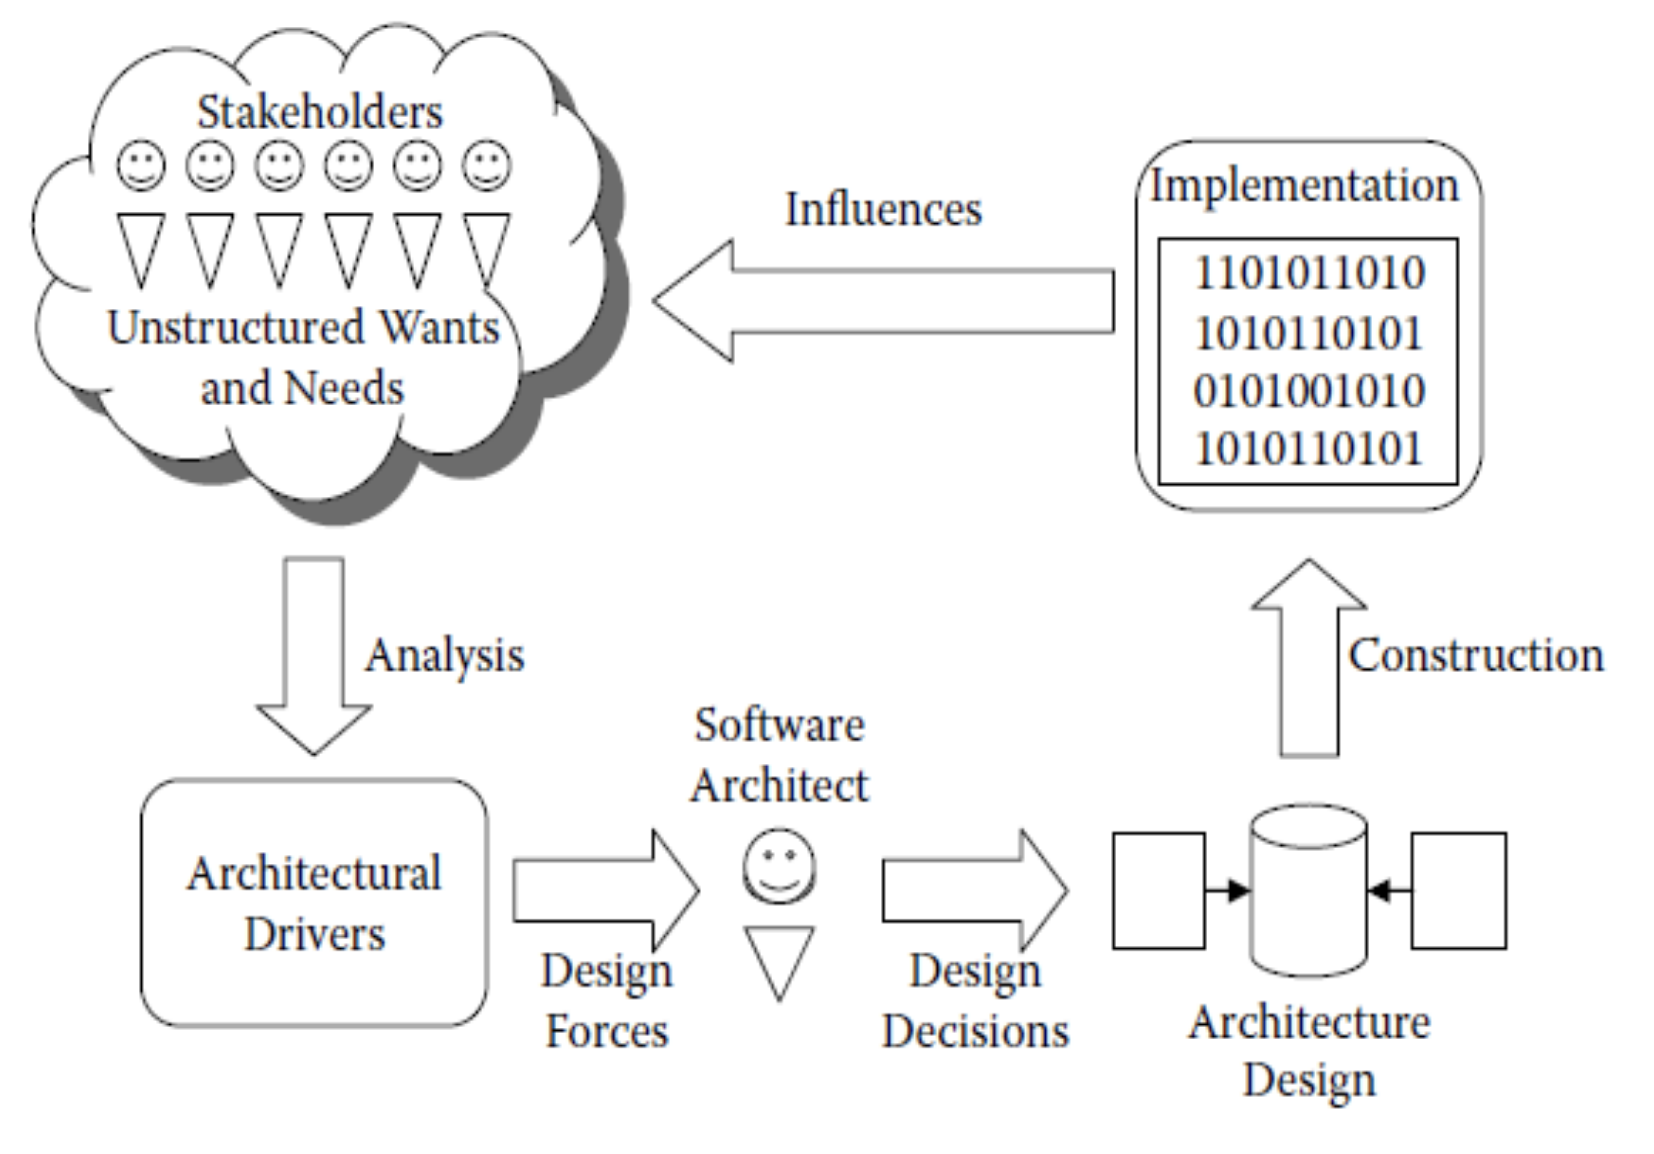
\includegraphics[width=220px]{sa_creation_process.png} \end{center}

Процесът на проектиране представлява циклично изпълнение на последователност от стъпки, в следствие на което се изгражда дадена софтуерна архитектура.
\bigbreak

В началото се избират целите (изисквания) с най-висок приоритет, които се превръщат в use-case или качествени сценарии.
Това са така наречените \textbf{driver}-и на архитектура, като се избират не повече от 10.
\bigbreak

След като driver-ите бъдат избрани се пристъпва към проектиране.
По време на проектиране могат да излезнат други питанки, които да доведат до промяна на драйверите и така да се зацикли до безкрайност.

\subsection{Избор на подходящи структури}

Структурата, която се получава директно от този подход, е \textbf{декомпозиция на модулите}.
В зависимост от driver-ите, наличните ресурси и приоритетите на заинтересованите лица се избират и други подходящи структури за документиране.

\subsection{Последователност на създаване на архитектурата}

Ще разгледаме \textbf{Attribute-Driven Design (ADD)} като подход за проектиране.
Той е рекурсивен процес на дефиниране на архитектурата, като на всяко ниво на задълбаване основна роля играят качествените изисквания.
Крайният резултат от \textbf{ADD} е първоначалната декомпозиция на модулите.
\bigbreak
\textbf{ADD} приема следните входни данни:
\begin{itemize}
    \item функционални изисквания, като сценарии за употреба (use-cases)
    \item функционални ограничения (constraints)
    \item качествени сценарии
\end{itemize}

Той включва следните стъпки:
\begin{enumerate}
    \item \textit{Избира се модул за декомпозиция}.
    \item \begin{enumerate}
        \item \textit{Избират се архитектурните driver-и}, които се отнасят за модула
        \item \textit{Избира се архитектурния модел на модула}, чрез избор и конфигурация на тактики за осъществяване на driver-ите.
        \item \textit{Създаване на подмодулите} спрямо избрания модел
        \item \textit{Приписване на функционалност на подмодулите}
        \item \textit{Създаване на други структури за подмодулите} (напр. на процесите)
        \item \textit{Дефиниция на интерфейсите на подмодулите}
        \item \textit{Проверява се декомпозицията}, дали отговаря на изискванията.
    \end{enumerate}
    \item \textit{Задълбаваме рекурсивно} ако има нужда от още детайлизация на някои подмодули.
\end{enumerate}


\section{Тактики}

\textbf{\textit{Тактиката}} е архитектурно решение, чрез което се контролира
резултата на даден сценарий за качество. Наборът от конкретни
тактики се нарича \textbf{\textit{архитектурна стратегия}}.
Конфигурация от тактики оформя \textbf{архитектурен модел}.

\subsection{Тактики за изправност}

\subsubsection{Откриване и предпазване от откази}
\begin{itemize}
\item \textit{Ping/Echo, Healthcheck} - компонент A пуска сигнал до компонент Б и очаква отговор в рамките на определен интервал от време.
\item \textit{Heartbeat, Keepalive} - компонент периодично изпраща сигнал, който друг компонент очавка.
\item \textit{Изключения} – обработват се изключения, които се генерират, когато се стигне до определено състояние на отказ.
\end{itemize}
\subsubsection{Отстраняване на откази}
\begin{itemize}
\item \textit{Активен излишък} - активно дублиране и поддържане в едно състояние на важните компоненти. Downtime за msec.
\item \textit{Пасивен излишък} - активниият компонент реагира на събитията и синхронизира резервните. Downtime за sec до hours.
\item \textit{Резерва (Spare)} - поддръжка на резервни изчислителни мощности. Downtime за min до hours.
\item \textit{Извеждане от употреба} - спиране на компонет за избягване на сривове. Например за предпазване от mem-leaks.
\item \textit{Следене на процесите (Process monitoring)} - процес следи други процеси, които ако откажат се преинициализират.
\end{itemize}
\subsubsection{Повторно въвеждане в употреба}
\begin{itemize}
\item \textit{Паралелна работа (shadow mode)} - компопент, който е бил счупен, се оставя да поработи за известно време в паралел с другите компоненти, преди да бъде въведен обратно.
\item \textit{Ре-синхронизация на състоянието}
\item \textit{Контролни точки и rollback} - при счупване, системата се възобновява (rollback) до последно запомненото консистентно състояние (checkpoint).
\end{itemize}

\subsection{Тактики за производителност}

\subsubsection{Намаляване на изискванията}
\begin{itemize}
\item \textit{Увеличаване на производителността на изчисленията}
\item \textit{Премахване на overhead} от ненужни изчисления
\item \textit{Промяна на периода} на настъпване на периодични събития
\item \textit{Промяна на тактовата честота (rate limiting)} - пропускаме само част от събитията когато не можем да променим периода на идването им. 
\item \textit{Опашка с краен размер} - аналог на leaky bucket алгоритъма.
\end{itemize}

\subsubsection{Управление на ресурсите}
\begin{itemize}
\item \textit{Паралелна обработка} на заявките
\item \textit{Излишък на данни/процеси} - cache, load-balancing и други.
\item \textit{Включване на допълнителни ресурси} - повече/по-мощен хардуер.
\end{itemize}

\subsubsection{Арбитраж на ресурсите}
Когато има недостиг на ресурси (т.е. спор за тях), трябва да има институция, която да решава (т.е. да извършва арбитраж) кое събитие да се обработи с предимство. Това се нарича \textbf{scheduling}. 

\subsection{Тактики за изменяемост}

Тактиките за изменяемост са:
\begin{itemize}
    \item \textit{Локализиране на промените} (намалява броя на директно засегнатите модули)
    \item Предотвратяване \textit{ефекта на вълната} (напр. open-closed принципа)
    \item \textit{Отлагане на свързването} при внедряване.
\end{itemize}

\subsection{Тактики за сигурност}

Тактикте за сигурност са:
\begin{itemize}
    \item \textit{Устояване} на атаките (doorlock)
    \item \textit{Откриване} на атаките (alarm)
    \item \textit{Възстановяване} след атака (застраховка)
\end{itemize}

\subsection{Тактики за изпитаемост (Testability)}

Testability тактиките са:
\begin{itemize}
    \item \textit{Запис и възпроизвеждане} на информацията, която минава през даден интерфейс
    \item \textit{Разделяне на интерфейса от реализацията}, за да може да се mock-ва реализацията
    \item \textit{Специализиран интерфейс за тестване} (напр. mock server)
    \item \textit{Вградени модули за мониторинг} (напр. излъчване на метрики към интерфейс)
\end{itemize}

\section{Архитектурни стилове}

Архитектурният стил дефинира семейство от системи чрез използването на
шаблон за структурна организация.
Стиловете обуславят речника на компонентите и конекторите, използвани в тях, както и ограниченията в начина на употребата им, напр. Топологията и семантиката на изпълнението им.

\subsection{Pipe-and-filter}

\begin{center} 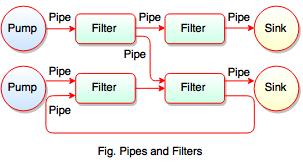
\includegraphics[width=220px]{pipe_and_filter.jpg} \end{center}

Модулите се делят на \textbf{филтри, канали, източник на данни и консуматор на данни}.
Каналите са потоци от данни изпълняващи ролята на конектори между филтрите.
Филтрите са модули, трансформиращи входните си данни, които могат да работят паралелно и независимо едни от други, като всеки филтър започва да предава изходните данни към следващия филтър преди да е свършил с обработката на всичките данни.
Този начин за обработка на данни позволява паралелизъм (конвейеризация).
\bigbreak
Филтрите нямат никаква информация за съседите си, което прави архитектурата \textbf{гъвкава и лесна за разбиране}.
От друга страна, производителността \textbf{страда заради parse-ването} на данни от всеки филтър.

\subsection{Layered}
Тук компонентите са вертикално разделени на слоеве, като всеки слой може да предлага услуги на слоя над себе си и да използва услугите на слоя под себе си.
Може да разгледаме този стил като разширение на клиент-сървър архитектурата - всеки слой е клиент за слоя под себе си и сървър за слоя над себе си.
\bigbreak
Предимствата включват \textbf{абстракция и лесна изменяемост}, докато недостатъците включват \textbf{компромиси с производителността} поради стриктните правила на комуникация, както и \textbf{по-сложен дизайн процес}.

\subsection{Client-server}
\begin{center} 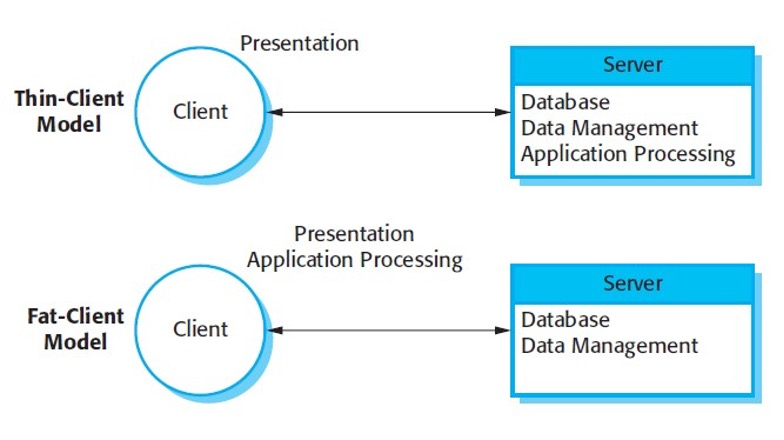
\includegraphics[width=250px]{client_server.jpg} \end{center}

Системата е построена като набор от сървъри, предлагащи услуги, и клиенти, които използват тези услуги. Клиентите могат да бъдат “тънки” или “дебели” - дебелите имплементират част от функционалността, а тънките - единствено потребителския интерфейс.
\bigbreak
Предимствата на този стил са \textbf{централизираните данни и сигурността}, а недостатъците - \textbf{риск от претоварване}, както и \textbf{нужда от резерви в случай на server failure}.

\subsection{Repository/Blackboard}
\begin{center} 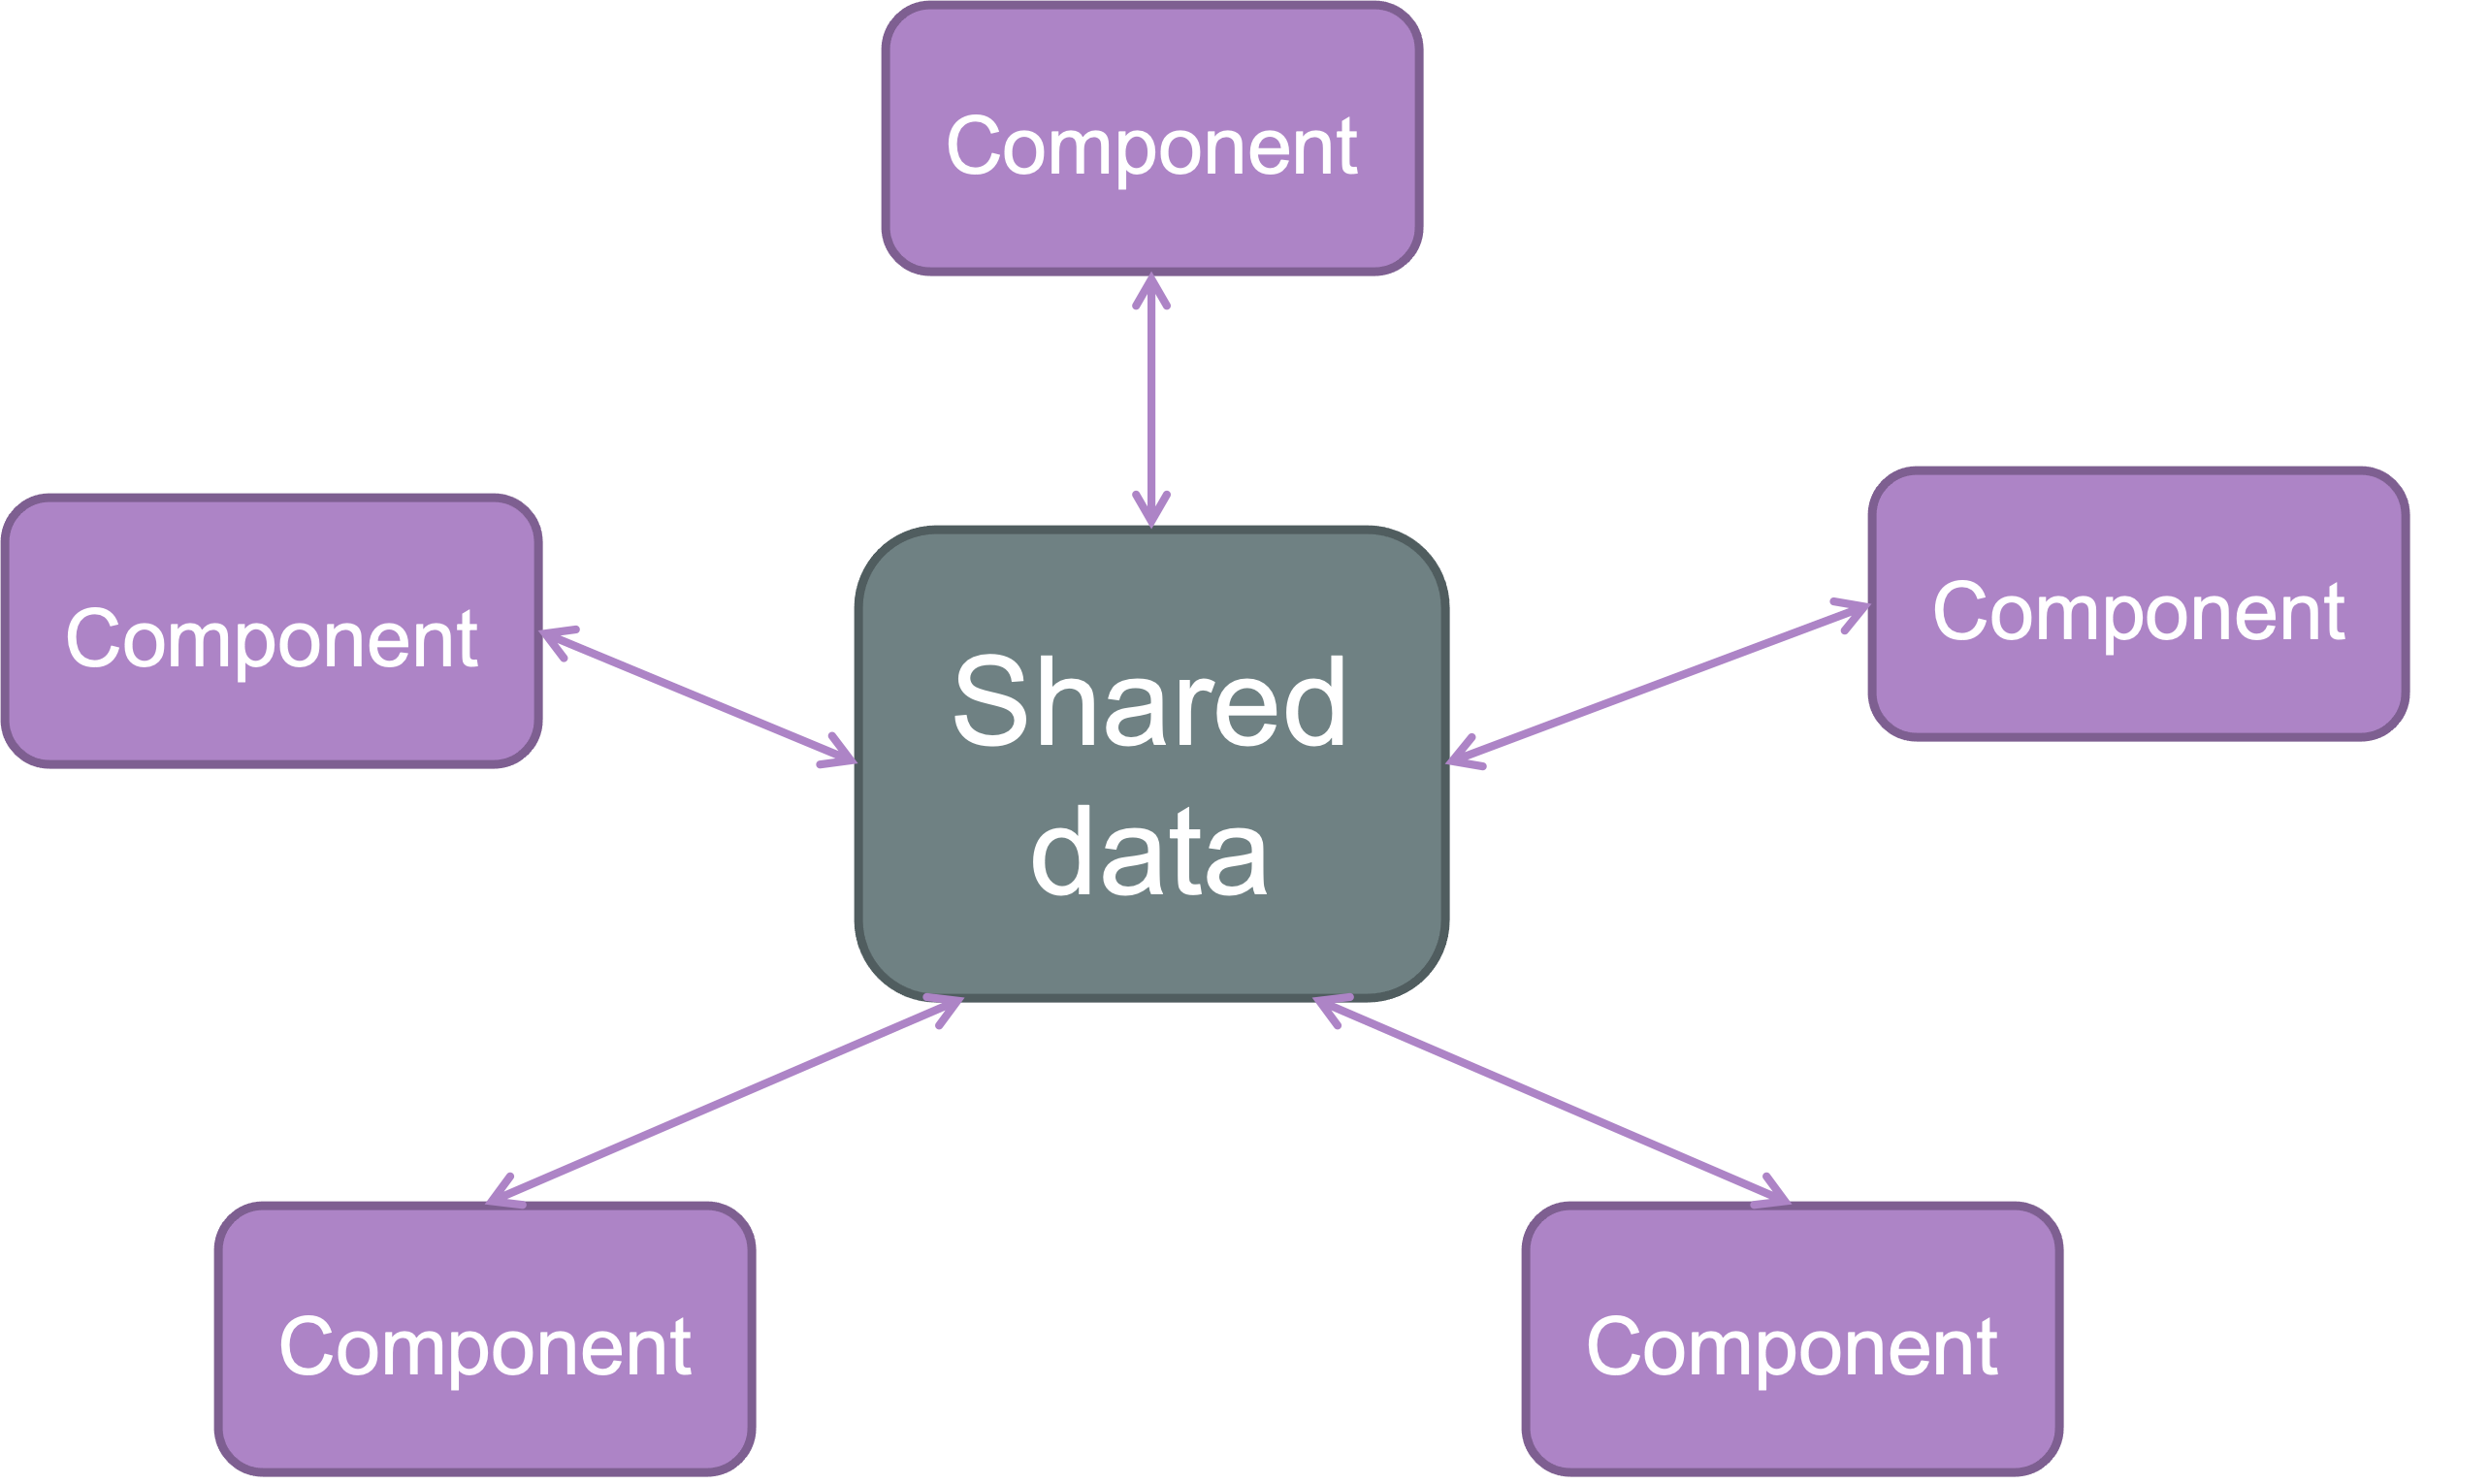
\includegraphics[width=250px]{shared_memory.png} \end{center}

Repository и Blackboard са две вариации на архитектурния стил “споделени данни”.
Тук данните могат да се разглеждат като конектор между компонентите (агентите).
При repository вариацията, когато се изпратят данни към общия конектор, всички агенти биват уведомени.
При blackboard вариацията инициативата е на модула с данните, а агентите се абонатиза събития (event listeners).
\bigbreak
Предимствата на този стил включват \textbf{скалируемост} - компоненти се добавят лесно, и висока ефективност при размяна на голямо количество данни.
От друга страна, споделената памет представлява \textbf{bottleneck} при голямо количество компоненти и заявки, също така е \textbf{трудна за имплементация} при разпределени системи.

\subsection{Model-View-Controller}
Състои се от:
\begin{itemize}
    \item \textbf{модел} - изпраща данни към изгледа, приема заявки за промяна на данните и управлява операциите с тях.
    \item \textbf{изглед} - управлява презентацията на данните пред потребителите.
    \item \textbf{контролер} - отговаря за взаимодействието с потребителя - натискане на клавиш, кликване и т.н., като изпраща заявки към модела и изгледа за необходимите действия
\end{itemize}

Този стил прави системата \textbf{гъвкава и разширяема}, но добавя \textbf{много сложност към архитектурата}, както и може да доведе до \textbf{компромиси с производителността}.

\subsection{Implicit invocation/Message passing}
\begin{center} 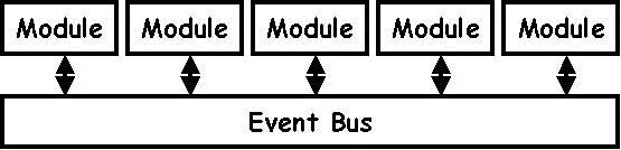
\includegraphics[width=300px]{implicit_invocation.jpg} \end{center}

При този стил компонентите си комуникират чрез т.нар. “Събития”. Тези събития може да съдържат както контролни съобщения, така и данни. Компонентите при такава архитектура работят паралелно, а конектора между тях е шина, по която се предават събитията.
\bigbreak
Предимствата включват \textbf{сигурност}, както и \textbf{гъвкавост (loose coupling на компонентите)}.
Недостатъците са \textbf{компромис с надеждността (ако шината умре)}, както и \textbf{несигурност} (ами ако няма компонент, който да отговори на дадено събитие).

\section{Документиране на софтуерната архитектура}

\subsection{Предназначение на документацията}
Документирането на СА е въпрос на документиране на всички съставляващи я структури поотделно.
Документацията е от важност с оглед на това да може в бъдеще системата да бъде лесно поддържана, безпроблемно изменяна и ясно разказвана на клиенти, потребители.
Трябва да е достатъчно абстрактна, така че да бъде разбрана от нови служители, но и достатъчно детайлна, че да послужи за основа на проектирането. 
\bigbreak
Документите, предназначени за едни лица са различни от тези за други.
Най-често се създава набор от документи с обогатено съдържание, което указва къде каква информация се съдържа.

\subsection{Основен принцип на документацията}

Документацията се състои от описание на различните структури и когато тя се пише се мисли най-вече кой ще я чете.
Технописецът трябва да се поставя на мястото на четящия.
В документацията \textbf{различните структури може да се групират по различни начини} в зависимост от това, за \textbf{кого конкретно е предназначена съответната документация}.

\subsection{Съдържание на документацията}
Няма изграден индустриален стандарт за съдържанието на документацията на дадена структура. Тук разглеждаме 7-елементно съдържание, доказано в практиката

\begin{enumerate}
\item \textbf{\textit{Първично представяне}} -  обикновено графично, често UML, само с първостепенна информация.
\item \textbf{\textit{Описание на елементите и връзките}} - детайлно описание на елементите и връзките + второстепенни детайли. Следва да се опише смисъла и ролята на всеки един елемент и връзка, както и поведенията и интерфейсите на елементите.
\item \textbf{\textit{Описание на обкръжението}} - информация за това как елементите от документираната структура си взаимодействат с обкръжението – други системи, интерфейси, протоколи и т.н.
\item \textbf{\textit{Описание на възможните вариации}} - често архитектурата е изградена така, че да позволява варианти за някои от детайлите, като конкретния вариант може да бъде избран на по-късен етап. Обикновено се дават като ограничителни условия и изисквания. Трябва да бъдат описани вариантите и условията.
\item \textbf{\textit{Архитектурна обосновка}} - обяснява на заинтересованите лица защо структурата е проектирана по начина по който е описана. Обоснование на взетите решения, алтернативи, резултати, предположения.
\item \textbf{\textit{Терминологичен речник}} - кратко описание на използваната стандартна и нововъведена терминология.
\item \textbf{\textit{Допълнителна информация}} - всичко останало, административна информация. Съдържа описание на съдържанието си.
\end{enumerate}

\subsection{Избор на структури, които да бъдат документирани}
Различните перспективи преследват различни цели и имат различно предназначение.
Кои структури ще бъдат документирани зависи от това, кой ще чете документацията
\bigbreak

Алгоритъм за избор на структури е:
\begin{enumerate}
    \item \textbf{Създава се таблица} с разпределение на приоритетите на различните ЗЛ по различни изгледи
    \item \textbf{Комбинират се перспективите} за да се намали броя им (напр. декомпозиция + слоеве, процеси + внедряване и др.)
    \item \textbf{Задават се приоритети} на различните перспективи.
\end{enumerate}

\end{document}
